\chapter{Chapter 4 : Change point detection in left censored observations}\label{chp:4}

\minitoc

Faced with the singular characteristics of the data presented in Chapter \ref{chp:3}, it is interesting to set up methods for an automatic detection of relevant signals in order to support expert analysis. Left censored data are characteristic of concentration records due to the inherent limits of qualification (LOQ) in the sample analysis. In this chapter, a new framework is proposed in order to detect changepoints in left censored signals. The model used to describe the data involves a left censored Weibull distribution. A changepoint detection method is derived from such modeling. We propose the pruned exact linear time (PELT) search method to do so. We will show that theoritical assumptions are met in the context of left censored data for both the convergence of our estimator and the use of the PELT algorithm. Experiments on simulated datasets are carried out, and the proposed approach is compared with related method. The issue of the LOD and of the LOQ has been addressed here by supposing that the data was left-censored, and that the censoring threshold, the LOQ, is a known constant. This approach is rather common in concentration monitoring studies, and is referred to as an upper bound configuration [8]. To our knowledge, using changepoint detection on left-censored distributions for analysing pollutant concentration represents a new contribution to the field. 

\section{Model}

In the following, let us suppose that one has a series of observed data $y_1,\dots,y_n$, which is the outcome of a random vector $Y_1, \dots, Y_n$. The variables $Y_i$ are recorded sequentially, although the recording times are not necessarily equidistant. Thus, the indices in $Y_i$ are only indicators of the order of appearance in the sample, and not of the observation times. Furthermore, $Y_i$ are supposed to be independent. We are interested here in left-censored Weibull distributions, where the censoring threshold in known and fixed, and where potential changes in the scale parameter of the Weibull distributions may occur independently. In this chapter, we will suppose that the shape parameter $\sigma$ is known and invariant in time. The case where this parameter is unknown is treated in Chapter \ref{chp:5}. The definition of the true model writes as follows:

\begin{definition}
Suppose that $Y_{1}, ..., Y_{n}$ are independent random variables, such that $Y_{i}$ is a left-censored Weibull distribution, depending on a censoring threshold $a>0$ ($a$ is supposed to be known and fixed throughout) and on some shape parameter $\sigma$ and a scale parameter $\lambda_{k}^{\star}\in \Theta\subset ]0,\infty[$, for $t_{k-1}^{\star}\le i \le t_{k}^{\star}$, $k =1,..., K^{\star}$. The c.d.f. of  $Y_{i}$ is
\begin{equation}\label{eq:cdf-censored}
   F_{Y_{i}}(x) =  F(x;\lambda_{k}^{\star},\sigma)  = \left( 1-e^{-(\lambda_{k}^{\star}x)^\sigma}\right)\mathbbm{1}_{\lbrace x \geq a\rbrace } \ , 
\end{equation}
The vector $\bm t^{\star} = (0=t^{\star}_{0}<t^{\star}_{1}<...<t^{\star}_{K^{\star}-1}<t^{\star}_{K^{\star}-1}=n)$ is the vector containing the change-points, and $\bm \lambda^{\star} = (\lambda_{1}^{\star}, ..., \lambda_{K^{\star}}^{\star})$ is the vector of parameters associated to the $K^{\star}$ regimes. 
\end{definition}

In general, $K^{\star}$, $\bm t^{\star} $ and $\bm \lambda^{\star}$ are all unknown and one would estimate them starting from the data $y_{1}, ..., y_{n}$. Estimation will be carried out by minimising a contrast function (can also be desiganted by the term cost function), which would be the -log-likelihood in this framework. In the subsequent, we will consider two separate cases, according to whether the number of regimes $K^{\star}$ is priorly known or not. 

\subsection{Estimating change-points locations with  \texorpdfstring{$K^{\star}$}{K*} known}

First, we shall consider the case where the number of regimes is known, and one looks for the estimates of $t^\star_{k}$, $k=1,...,K^{\star}-1$ and  $\lambda_{1}^\star, ..., \lambda_{K^{\star}}^{\star}$. We define the following criterion, based on the negative log-likelihood of the observed sample : 
\begin{equation}\label{eq:crit-known-k}
  \CC_{Y_{1:n}}(\bm t, \bm \lambda ) = \sum_{k=0}^{K^{\star}-1}W(Y_{(t_{k}+1) : t_{k+1}}, \lambda_{k})  =  \sum_{k=0}^{K^{\star}-1} \sum_{i=t_{k}+1}^{t_{k+1}}-\ln f(Y_{i};\lambda_{k},\sigma) , 
\end{equation}
where $Y_{u:v}=(Y_{u},...,Y_{v})$, $\bm t=(0=t_{0}< t_{1}< ...< t_{K^{\star}}=n)$ and $\bm \lambda = (\lambda_{1}, ..., \lambda_{K^{\star}})\in \Theta^{K^{\star}}$, and 
\begin{equation}\label{eq:cens-dens}
  f(Y_{i};\lambda_{k},\sigma) = \bigg(1-e^{-(\lambda_{k}a)^\sigma}\bigg)^{\mathbbm{1}_{\lbrace Y_{i} = a\rbrace }} \bigg(\sigma\lambda_{k} (\lambda_{k}Y_i)^{\sigma-1} e^{-(\lambda_{k} Y_i)^\sigma}\bigg)^{\mathbbm{1}_{\lbrace Y_{i} > a\rbrace}} \ .
\end{equation}

If one denotes 
\begin{equation}\label{eq:vector-t}
  \TT_{K^{\star}} = \left\{  \bm t = (t_{0}, ..., t_{K^{\star}}),  0=t_{0}<t_{1}<...<t_{K^{\star}-1}<t_{K^{\star}}=n \right\} , 
\end{equation}
the set of all possible partitions of $Y_{1}, ..., Y_{n}$ into $K^{\star}$ regimes, then, the maximum likelihood estimates of  $\bm t^{\star}$ and $\bm \lambda^{\star}$ are defined as the quantities realising
\begin{equation}\label{eq:ml-known-k}
 (\hat{\bm t}, \hat{\bm \lambda})  = \arg \min_{\bm t\in  \TT_{K^{\star}} , \bm \lambda\in \Theta^{K^{\star}}}  \CC_{Y_{1:n}}(\bm t, \bm \lambda ) 
\end{equation}

In the following, we'll consider a slightly different writing of this optimisation problem. Let us define the maximum likelihood estimate in the segment $Y_{(t_{k}+1) : t_{k+1}}$ by :
\begin{equation}\label{eq:ml-expo}
\tilde \lambda_{k} = \arg \min_{\lambda\in\Theta}   \sum_{i=t_{k}+1}^{t_{k+1}}-\ln f(Y_{i};\lambda_{k},\sigma) \ ,
\end{equation}

where 
\begin{equation}\label{eq:ml-wei-1}
\sum_{i=t_{k}+1}^{t_{k+1}}\ln f(Y_{i};\lambda_{k},\sigma)  = \sum_{i=t_{k}+1}^{t_{k+1}}\ln\left(1-e^{-(\lambda_{k}a)^\sigma}\right)\mathbbm{1}_{\lbrace Y_{i} = a\rbrace }+\sum_{i=t_{k}+1}^{t_{k+1}}\bigg(\ln(\sigma\lambda_{k}) + (\sigma-1)\ln(\lambda_{k}Y_i) -(\lambda_{k} Y_i)^\sigma\bigg)\mathbbm{1}_{\lbrace Y_{i} > a\rbrace}, 
\end{equation}
%$n_{k}=t_{k+1}-t_{k}+1$ is the number of data in subsample $Y_{(t_{k}+1) : t_{k+1}}$, and $n_{k,a}$ is the number of uncensored data in the same subsample. 

In this case, by plugging $\tilde \lambda_{k}$ in Eq. \ref{eq:ml-known-k}, the initial optimisation problem is reduced to computing $\hat{\bm t}$, 
\begin{equation}\label{eq:ml-known-k-plugged}
 \hat{\bm t} = \arg \min_{\bm t\in  \TT_{K^{\star}} }  \CC_{Y_{1:n}}(\bm t, \tilde{\bm\lambda} ) = \arg \min_{\bm t\in  \TT_{K^{\star}} } \sum_{k=0}^{K^{\star}-1}W(Y_{(t_{k}+1) : t_{k+1}}, \tilde\lambda_{k}) 
\end{equation}

Several remarks may be made at this point. First, one should notice that Eq. \ref{eq:ml-expo} may not be explicitly solved. Nevertheless, one may check that second derivative with respect to $\lambda_{k}$ is strictly positive, ensuring the existence of a minimum. The illustration is provided in Appendix \ref{app:chap4}. From a practical point of view, in the numerical implementation to be presented in the next sections, a Newton-Raphson approach will be used for computing $\tilde \lambda_{k}$. Second, the search for $ \hat{\bm t}$ in Eq. \ref{eq:ml-known-k-plugged} would normally require a $\OO(n^{K^{\star}-1})$, but we will reduce it to at most a quadratic one, using dynamical programming and other heuristics. 

The estimate $\hat{\bm t}, \hat{\bm \lambda}$ may be shown to have consistency properties. In order to establish them, some further notations and hypotheses are being needed. 
\begin{itemize}
\item[\textbf{(H1)}] $\Theta$ is compact and there exists $\Delta_{\bm \lambda}^{\star}>0$ such that $\vert \lambda_{k}^{\star}-\lambda_{k-1}^{\star}\vert > \Delta_{\bm \lambda}^{\star}$, for all $k=2,...,K^{\star}$. 
\item[\textbf{(H2)}] If one denotes $\tau^\star_k = \frac{t^\star_{k}}{n}$, $k=0,...,K^{\star}$, the normalized configuration, then $\tau^\star_k$ is constant when the sample size $n$ varies, for all $k=0,...,K^{\star}$. 
\item[\textbf{(H3)}]  There exists $\Delta_{\bm \tau}^{\star}>0$ such that $\vert \tau_{k}^{\star}-\tau_{k-1}^{\star}\vert > \Delta_{\bm \tau}^{\star}$, for all $k=1,...,K^{\star}$.
\end{itemize}

The first hypothesis mainly aims at ensuring sufficient conditions for the identifiability of the model, by imposing a minimum gap between two consecutive $\lambda$'s. The second hypothesis, which is also the strongest one, implies that change-point locations are independent of the scale and frequency at which the data is sampled. This hypothesis will also allow us to derive the asymptotic behaviour of the estimate, when the sample size is sufficiently large. One should note here that a larger sample means a finer scale for sampling the data and not an extension of the period of observation. Eventually, the third hypothesis checks that each regime contains sufficient data for obtaining reliable estimates for the $\lambda$'s. 

With the above notations and definitions, one may state the following result:

\begin{proposition}
Under the hypotheses (H1)-(H3), the maximum likelihood estimate is weakly consistent
\begin{equation}\label{eq:ml-convergence}
  (\hat{\bm \tau}, \hat{\bm \lambda}) \xrightarrow[n\rightarrow \infty]{\PP^{\star}}   (\bm \tau^{\star}, \bm \lambda^{\star}) \ ,
\end{equation}
where  $\hat{\bm t}$ and $\hat{\bm \lambda}$ are computed by solving Eq. \ref{eq:ml-known-k-plugged} and \ref{eq:ml-expo}, and $\hat{\bm \tau}= \frac{\hat{\bm t}}{n}$ is the estimate of the normalized configuration.
\end{proposition}

This proposition is a particular case of Theorem 2.2 in \cite{Lavielle1997}. A detailed proof checking that hypotheses (H1)-(H3) are sufficient is provided in Appendix \ref{app:chap4}. 

Not only is the maximum likelihood consistent, but one may equally derive its consistency rate: 

\begin{proposition}
Under the hypotheses (H1)-(H3), $\lbrace n\Vert \hat{\bm \tau} - \bm\tau^{\star}\Vert_{\infty}\rbrace$ and $\lbrace \sqrt n\Vert \hat{\bm \lambda} - \bm\lambda^{\star}\Vert_{\infty}\rbrace$ are uniformly tight in probability:
\begin{equation}\label{eq:ml-rate}
\begin{split}
  \lim_{\delta\rightarrow \infty} \lim_{n\rightarrow \infty} \PP^{\star}\left( n\Vert \hat{\bm \tau} - \bm\tau^{\star}\Vert_{\infty} \ge \delta \right) = 0 \\
   \lim_{\eta \rightarrow \infty} \lim_{n\rightarrow \infty} \PP^{\star}\left( \sqrt n\Vert \hat{\bm \lambda} - \bm\lambda^{\star}\Vert_{\infty} \ge \eta \right) = 0  .
  \end{split}
\end{equation}
\end{proposition}


\subsection{Estimating change-points locations with  \texorpdfstring{$K^{\star}$}{K*} unknown}

In practice, $K^{\star}$ will be most often unknown, and one will need to estimate it also. In this case, one may define a penalised criterion, 
\begin{equation}\label{eq:crit-unknown-k}
 \tilde \CC_{Y_{1:n}}(K, \bm t, \bm \lambda ) = \sum_{k=0}^{K^{\star}-1}W(Y_{(t_{k}+1) : t_{k+1}}, \lambda_{k}) + \beta_{n}K \ , 
\end{equation}
where $\beta_{n}$ is a positive sequence.

We follow the same approach as  in \cite{Lavielle1997} to prove that under some further usual assumptions on $\beta_{n}$, the estimates obtained by minimising the penalised criterion in Equation \ref{eq:crit-unknown-k} are consistent. 

First of all, let us assume that $K^{\star}$ is bounded from above, that is there exists some $K_{\max}\in \NN$, such that $K^{\star} \le K_{\max}$. Equivalently, one may suppose that there exists a minorant of $\Delta_{\bm \tau}^{\star}$:
\begin{itemize}
\item[\textbf{(H4)}] There exists $\Delta_{\bm \tau}>0$, such that $\Delta_{\bm \tau}^{\star} > \Delta_{\bm \tau}$. In this case, the maximum number of regimes may be written as $K_{\max} = \frac{1}{\Delta_{\bm \tau}}$. 
\end{itemize}

For each $K=1,..., K_{\max}$, define the set of possible configurations:
\begin{equation}\label{eq:vector-tau}
  \TT_{K}^{\Delta} = \left\{  \bm \tau = (0=\tau_{0}<\tau_{1}< ...<\tau_{K-1}<\tau_{K}=1),  \right. \\
 \left. \tau_{k}-\tau_{k-1}\ge \Delta_{\tau}, \forall k=1,...,K \right\} . 
\end{equation}

The penalised maximum-likelihood estimate may be written 
\begin{equation}\label{eq:ml-unknown-k}
 (\hat K, \hat{\bm \tau}, \hat{\bm \lambda})  = \arg\min_{K=1,...,K_{\max}} \min_{\bm \tau\in  \TT_{K}^{\Delta} , \bm \lambda\in \Theta^{K}}   \tilde \CC_{Y_{1:n}}(K, \lfloor n\bm \tau \rfloor, \bm \lambda )  \ , 
\end{equation}
with $\tilde \CC_{Y_{1:n}}(K, \lfloor n\bm \tau \rfloor, \bm \lambda )$ defined as in Eq. \ref{eq:crit-unknown-k}. 

Consistency of the penalised estimate may be shown by introducing one more hypothesis. 
\begin{itemize}
\item[\textbf{(H5)}] The sequence $\beta_{n}$ verifies $\beta_{n}\xrightarrow[n\rightarrow \infty]{} \infty$ and $\frac{\beta_{n}}{n}\xrightarrow[n\rightarrow \infty]{} 0$.
\end{itemize}

The latter hypothesis is checked by a large palette of penalties, including the BIC criterion, $\beta_{n}=\frac{\ln n}{2}$. 

\begin{proposition}
Under the hypotheses (H1)-(H5), the penalised maximum-likelihood estimate defined in Eq. \ref{eq:ml-unknown-k} is weakly consistent
\begin{equation}\label{eq:ml-convergence-pen}
  (\hat K, \hat{\bm \tau}, \hat{\bm \lambda}) \xrightarrow[n\rightarrow \infty]{\PP^{\star}}   (K^{\star}, \bm \tau^{\star}, \bm \lambda^{\star}) \ .
\end{equation}
\end{proposition}

The proof of this assertion is a direct consequence of Theorem 3.1 in \cite{Lavielle1997}. 

%\subsection{Extension to the multi-threshold case}

%In practise, the censoring threshold in the data is not fixed in time. The heterogeneity of the stations' measurement equipment was discussed in Chapter \ref{chp:3}. Theoretically, this means implies that multiple thresholds the modelling must be considered in the modelling,take into account several thresholds which we will denote by the set $\mathcal{A} = {a_1,a_2,...,a_J}$ with $J$ being the number of different existing thresholds. The propositions made earlier in this section are also still correct in the context of multiple several thresholds. However, the formulation of the problem changes slightly. We now assume that $Y_1,\dots,Y_n$ are defined as follows:

%\begin{definition}
%Suppose that $X_{1}, ..., X_{n}$ and $Z_{1}, ...,Z_{n}$ are independent random variables. $X_i$ is a Weibull distribution depending on a shape parameter $\sigma$, a scale parameter $\lambda_{k}^{\star}\in \Theta\subset ]0,\infty[$, for $t_{k-1}^{\star}\le i \le t_{k}^{\star}$, $k =1,..., K^{\star}$. $Y_i$ is a Dirac measure on the set of all censoring threshold values $\mathcal{A} = {a_1,a_2,...,a_I}$. For all $i$, define $Y_i = \max(X_i,Z_i)$. The c.d.f. of  $Y_{i}$ is
%\begin{align*}
%   F_{Y_{i}}(x) &= \mathbbm{P}(Y_i \leq x) = \sum_{1\leq j \leq J}\mathbbm{P}(Y_i \leq x \cap Z_i = a_j) \\
%   &= \sum_{1\leq j \leq J}\left( 1-e^{-(\lambda_{k}^{\star}x)^\sigma}\right)\mathbbm{1}_{\lbrace x \geq a_j\rbrace }\delta_{} , 
%\end{align*}
%The vector $\bm t^{\star} = (0=t^{\star}_{0}<t^{\star}_{1}<...<t^{\star}_{K^{\star}-1}<t^{\star}_{K^{\star}-1}=n)$ is the vector containing the change-points, and $\bm \lambda^{\star} = (\lambda_{1}^{\star}, ..., \lambda_{K^{\star}}^{\star})$ is the vector of parameters associated to the $K^{\star}$ regimes. 
%\end{definition}

\section{Estimation procedure}\label{chp:4:2}

The model having been introduced and its theoretical properties established, one may now focus on its practical implementation. As the true number of change-points is seldom known for real datasets, the proposed algorithm considers the case where $K^{\star}$ is unknown. 

\subsection{Estimating the \texorpdfstring{$\lambda$}{l}'s}

First of all, one should be able to properly compute $\lambda_{s:t}$ as the estimate of the left-censored exponential parameter, given the sub-sample $Y_s,\dots,Y_t$. After having written the log-likelihood similarly to Eq. \ref{eq:ml-wei-1}, and computed the derivative with respect to $\lambda$, one may notice that the latter does not lead to an analytical expression for $\lambda_{s:t}$:

\begin{equation}\label{eq:ml-wei-d1}
\frac{\partial\sum_{i=t_{k}+1}^{t_{k+1}}\ln f(y;\lambda,\sigma)}{\partial \lambda} = \sum_{i=t_{k}+1}^{t_{k+1}}\frac{a^\sigma\sigma(\lambda)^{\sigma-1}e^{-(\lambda a)^\sigma}}{1-e^{-(\lambda a)^\sigma}} \mathbbm{1}_{\lbrace y = a\rbrace }+\sum_{i=t_{k}+1}^{t_{k+1}}\bigg(\frac{\sigma}{\lambda} - \sigma(\lambda)^{\sigma-1}y^{\sigma}\bigg)\mathbbm{1}_{\lbrace y > a\rbrace}, 
\end{equation}

Hence, instead of having an explicit formula for $\lambda_{s:t}$, one derives it through a numerical optimisation procedure. In the work presented here, the Newton-Raphson method was used to search for the zeros of the first derivate of the cost function in order to find its minimum. Furthermore, checking that the second derivative is strictly positive, thus guaranteeing the unicity of the maximum likelihood estimate, can prove to be a difficult task. This study is made in Appendix \ref{app:chap4}.

\begin{figure}[ht]
    \centering
    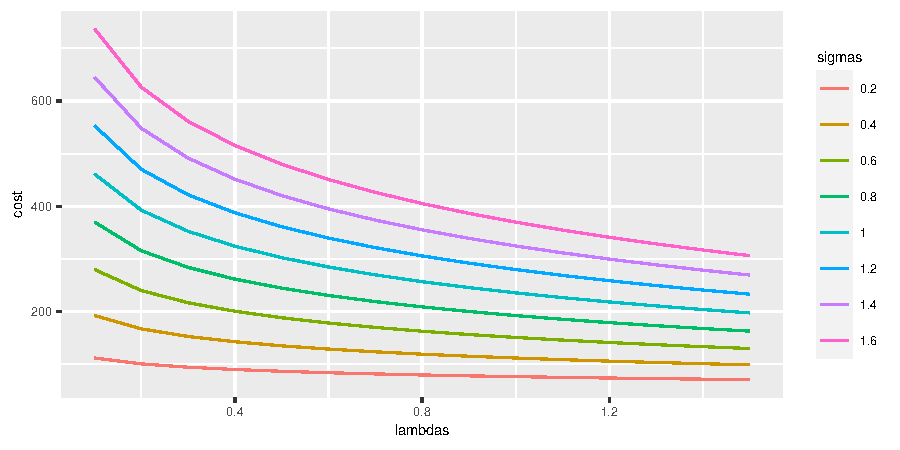
\includegraphics{figs/Chap4/only_cens.pdf}
    \caption{Plot of the cost function values against $\lambda$ values when all observations are censored. It is represented for several $\sigma$ values. The sample consists in 100 values of threshold $a = 0.1$.}
    \label{fig:onlycens}
\end{figure}

However, the case where all data in the sample $Y_s,\dots,Y_t$ are censored is an exception. Looking at the analytical likelihood formula, we find that the $\lambda$ realising the minimum of the cost function still exists, but tends toward infinity. This result is shown in Figure \ref{fig:onlycens} where We can see it is the case for any $\sigma$ value. To solve this problem from a computational point of view, we impose an upper bound on the possible values of lambda. In the remainder of this work, the maximum value of $\lambda$ is set to $10^6$. When the value of the estimate exceeds this threshold, the Newton-Raphson procedure terminates.

\subsection{Estimation procedure for \texorpdfstring{$K^{\star}$}{K*}, \texorpdfstring{$\bm t^{\star}$}{t*} and \texorpdfstring{$\bm \lambda^{\star}$}{l*}}\label{sub:pelt}

The estimation procedure aims at minimising the penalised log-likelihood in Eq. \ref{eq:crit-unknown-k}. The optimisation problem is equivalent to finding both the best partitioning of the data as defined by $\hat{K}$ and $\hat{\bm t}$, as well as the estimates for the scale parameters of the left-censored Weibull within each segment, $\hat{\bm \lambda}$. the complexity related to the search of the optimal partitioning is prohibitive in practice, several heuristics based on dynamic programming have been proposed in the literature \cite{Maidstone2016,Jackson2005,Jensen1969,Os2004}. The approach adopted here was the Pruned Exact Linear Time algorithm \cite{Killick2012} as introduced in Chapter \ref{chp:2}, which has the advantage of achieving a linear complexity in the number of data. Let's denote $F(s)$ for $s\in [1:n]$ the best segmentation found so far on the data $(y_1,...,y_s)$:  
$$F(s) = \max_{\bm{\mathcal{T}}\in\mathcal{T}_s}\bigg(\sum_{k=1}^{m+1}[W(Y_{(t_{k}+1) : t_{k+1}}, \lambda_{k}) - \beta_{n}]\bigg),$$
with $\mathcal{T}_s = \{\bm{t} :0 = t_0 < t_1 <...<t_m <t_{m+1} = s\}$  be the set of all possible segmentation of signal $y_{1:s}$. With these notations, the procedure may be written as illustrated in Algorithm \ref{algo:pelt}.

\begin{algorithm}
\caption{PELT algorithm combined with Newton-Raphson:}\label{algo:pelt}
\begin{algorithmic}

\State \textbf{input} : the data $y_{1},...,y_{n}$, the censoring threshold $a$,  and the penalty term $\beta_{n}$ \\
  
\State \textbf{initialisations} : $F(0)=\beta_{n}$, $R_{1}=\lbrace 0\rbrace$, $CP(0)=NULL$  \\
  
 \ForAll{$\tilde t=1,...,n$} :
 \begin{enumerate}
  \item Compute 
  $ F(\tilde t)=\min_{t\in R_{\tilde t}}\lbrace F(t)+W(y_{(t+1):\tilde t}, \hat \lambda_{(t+1):\tilde t})+\beta_{n}\rbrace $
  \item Compute $ \overline t=\arg \min_{t\in R_{\tilde t}}\lbrace F(t)+W(y_{(t+1):\tilde t}, \hat \lambda_{(t+1):\tilde t})+\beta_{n}\rbrace $ 
  \item Set $CP(\tilde t)=[CP(\overline t), \overline t]$
  \item Set $R_{\tilde t+1}=\left\{t\in R_{\tilde t}\cup \lbrace\tilde t\rbrace \vert F(t)+W(y_{(t+1):\tilde t}, \hat \lambda_{(t+1):\tilde t}) +\beta_{n} \le F(\tilde t)   \right\}$ 
 \end{enumerate} 
   \EndFor \\
   
\State \textbf{output} : the vector of change-points $CP$. 
 
\end{algorithmic}
\end{algorithm} 

The resulting algorithm is very similar to the one exposed in Chapter \ref{chp:2}. In Algorithm \ref{algo:pelt} however, the $\hat \lambda_{(t+1):\tilde t}$ is the output of the Newton-Raphson method, trained on $y_{t+1},...,y_{\tilde t}$. Let us mention here that Algorithm \ref{algo:pelt} relies on a series of hyper-parameters which ought to be tuned: the precision threshold and the maximum number of iterations in the Newton-Raphson step, the initial values for the $\lambda$’s in Newton-Raphson step also, and the minimum number of observations between two consecutive change-points. 

\section{Simulation study}

The model presented in the previous sections is subjected to a series of tests. The purpose of these tests is twofold: 

\begin{enumerate}
    \item As mentioned in Section \ref{chp:4:2}, our algorithm is driven by hyperparameters. We would like to be able to adjust these to achieve good performance.
    \item We would also like to develop a procedure to calibrate the penalty value and compare its performance with a method from the litterature. 
\end{enumerate}

To assess the good tuning and efficiency of our method, we will compare its performances with the \textit{MultRank} method developped by \cite{YutFong2011} presented in Chapter \ref{chp:2}. Since this method being also adapted for censored data, it constitutes a coherent reference point.  

\subsection{Tuning hyper-parameters of the Newton-Raphson method}

\begin{itemize}
    \item[$\blacksquare$] \textbf{Precision of the Newton-Raphson method:} the precision criterion in the Newton-Raphson algorithm implemented here is user-defined threshold $\epsilon$. If we denote $\hat\lambda_n$ the estimate obtained at the $n$-th iteration in the Newton-Raphson loop, the criterion can be written $\lvert \hat\lambda_{n+1} - \hat\lambda_n\rvert \leq \epsilon$. In other word, the method stops when the correction made to the estimate value at the $n$-th step is below $\epsilon$. The threshold $\epsilon$ is fixed at the value $10^{-8}$. (CITER UNe SOURCE POUR LES NORMES IEEE ?)
    \item[$\blacksquare$] \textbf{Initialisation value in the Newton-Raphson method:} four initialisation values are available in our implementation. We can choose between the classical techniques such as the moment method estimator $\lambda_{init}^{MM}$ \cite{Johnson1994}, the quantile inversion estimator $\lambda_{init}^{QI}$, the weighed maximum likelihood estimator $\lambda_{init}^{WMLE}$ \cite{sadani2019new} or the classical maximum likelihood estimator $\lambda_{init}^{MLE}$ of a Weibull scale parameter. Supposing a sample of observations $\bm x = (x_1,...,x_n)$ generated from a left censored Weibull of parameters $(\lambda,\sigma)$ and censoring threshold $a$, we can define them as follow : 
    %\begin{align*}
    \begin{itemize}
        \item[$\circ$] $\lambda_{init}^{MM} =\frac{\Gamma(1+\frac{1}{\sigma})}{\bar{\bm x}}$ 
        \item[$\circ$] $\lambda_{init}^{QI} = \frac{\bigg(-\ln(1-\alpha)\bigg)^{\frac{1}{\sigma}}}{q_{\bm x}^\alpha}$
        \item[$\circ$] $\lambda_{init}^{WMLE} = \bigg(\frac{1}{nq^{0.5}_{\mathcal{W}(n,n)}}\sum_{i = 1}^nx_i^\sigma \bigg)^{-\frac{1}{\sigma}}$
        \item[$\circ$] $\lambda_{init}^{MLE} = \bigg(\frac{1}{n}\sum_{i = 1}^nx_i^\sigma \bigg)^{-\frac{1}{\sigma}}$, 
    \end{itemize}
    %\end{align*}
    where $q^{0.5}_{\mathcal{W}(n,n)}$ is the median of Weibull with parameters $(n,n)$, $q_{\bm x}^\alpha$ is the $\alpha$-th empirical quantile of the sample $\bm x$. \\
     Two important points must be noted. First, all the initialisation values depend on $\sigma$. It is not problematic in our simulation tests because it is supposed known and fixed. However it stresses again the necessity of its estimation in the future (see Chapter \ref{chp:5}). Second, those estimators do not take the censorship into account. They are all biased (except if the sample $\bm x$ does not bear any censored values). \\
     We tested all possible configurations with the varying values of $n = (20,100,500)$, $\lambda = (1/100,1,100)$ and $a$ depending on a censoring rate $\alpha = (0.05,0.25,0.5,0.75,0.95)$. $a$ was the threshold such that $\alpha \%$ of the sample was censored. The shape parameter is supposed known and fixed at $\sigma = 0.5$. For each cases, we simulated $N = 1000$ samples of left censored Weibull with shape parameter $\lambda$ and censored rate $\alpha$. We then compute the mean of all estimates for each initialisation values. All the results are stored into Tables \ref{tab:sim:init1} and \ref{tab:sim:init2}. The simulations show that all initialisation values lead to extremely similar results. It is worth mentioning that the quantile is not reliable for low values of $n$. In the rest of this work, the initialisation value will be defined as the weighed maximum likelihood. The table for the case where $n = 500$ is not displayed because all methods gave the same results. However, the most important result of this experiment is that the method converges and that the choice of the initialization point is important. From now on, we choose to initialize the method with the weighed Maximum Likelihood Estimator. More experiences are provided in Appendix \ref{app:chap4}.
     \item[$\blacksquare$] \textbf{Maximum number of iteration in the Newton-Raphson method $N_{max}$:} this parameter is user-defined. When the Newton-Raphson method reaches $N_{max}$-th iteration, it stops. The following experience has been conducted to tune this parameter : 
    \begin{enumerate}
        \item Generate a $n$ sized sample $y_1,...,y_n$ following a left-censored Weibull with scale and shape parameters $\lambda$ and $\sigma$ and with censoring threshold $a$ censoring $\alpha \%$ of the sample. We chose $n=100$.
        \item Store the minimum iteration such that the estimate value $\hat\lambda$ does not evolve. The maximum iteration value allowed for the experiment is $N_{max} = 100$ 
        \item Repeat the two first step $N = 1000$ times.
        \item Compute the mean value of the minimum iteration and the mean values of the $N$ samples estimated parameters. 
    \end{enumerate}
    Several configurations are tested with different values of threshold $\alpha$ and $\lambda$. The shape parameter is fixed at $\sigma = 0.5$. We initialize the method with the Weighed Maximum Likelihood value. The results are stored in Table \ref{tab:sim:Nmax}. Looking at the average minimum iteration needed to reach a stable value, $N_{max}$ was set to 100 which seems a reasonable choice for the rest of this work. It can be noted that the minimum number of iterations needed for low values of $\lambda$ are higher than in other configurations  
\end{itemize}

\textbf{Summary of the simulations :} we calibrate the Newton-Raphson method the following way:
\begin{itemize}
    \item Precision threshold $\epsilon = 10^{-8}$. 
    \item Maximum number of iterations tolerated $N_{max} = 100$.
    \item Initialisation method : weighed Maximum Likelihood Estimator.
\end{itemize}

\begin{table}[ht] 
\centering
\begin{tabular}{|rr||rrrr|}
 \hline
 $\alpha$ & $\lambda$ & $\overline{\hat\lambda}_{WMLE}$ & $\overline{\hat\lambda}_{MLE}$ & $\overline{\hat\lambda}_{QI}$ & $\overline{\hat\lambda}_{MM}$ \\
  \hline
  \hline
 0.05 & 100.00 & 116.77 & 116.77 & 1963.08 & 116.77 \\ 
   0.05 & 1.00 & 1.16 & 1.16 & 1.47 & 1.16 \\ 
   0.05 & 0.01 & 0.01 & 0.01 & 1790.22 & 0.01 \\ 
   0.25 & 100.00 & 119.24 & 119.24 & 151.37 & 119.24 \\ 
   0.25 & 1.00 & 1.16 & 1.16 & 2362.08 & 1.16 \\ 
   0.25 & 0.01 & 0.01 & 0.01 & 6038.39 & 0.01 \\ 
   0.50 & 100.00 & 118.07 & 118.07 & 3687.48 & 118.07 \\ 
   0.50 & 1.00 & 1.18 & 1.18 & 1.48 & 1.18 \\ 
   0.50 & 0.01 & 0.01 & 0.01 & 0.02 & 0.01 \\ 
   0.75 & 100.00 & 122.44 & 122.44 & 1724.86 & 122.44 \\ 
   0.75 & 1.00 & 1.25 & 1.25 & 2602.37 & 1.25 \\ 
   0.75 & 0.01 & 0.01 & 0.01 & 1189.03 & 0.01 \\ 
   0.95 & 100.00 & 163.51 & 163.51 & 165.04 & 163.51 \\ 
   0.95 & 1.00 & 1.62 & 1.62 & 1.63 & 1.62 \\ 
   0.95 & 0.01 & 0.02 & 0.02 & 0.02 & 0.02 \\ 
   \hline
\end{tabular}
\caption{Choice of initialisitation value: simulation results for $n = 20$.}\label{tab:sim:init1}
\end{table}

\begin{table}[ht]
\centering
\begin{tabular}{|rr||rrrr|}
\hline
 $\alpha$ & $\lambda$ & $\overline{\hat\lambda}_{WMLE}$ & $\overline{\hat\lambda}_{MLE}$ & $\overline{\hat\lambda}_{QI}$ & $\overline{\hat\lambda}_{MM}$ \\ 
  \hline
  \hline
0.05 & 100.00 & 102.65 & 102.65 & 102.98 & 102.65 \\ 
  0.05 & 1.00 & 1.03 & 1.03 & 1.03 & 1.03 \\ 
  0.05 & 0.01 & 0.01 & 0.01 & 0.01 & 0.01 \\ 
  0.25 & 100.00 & 102.97 & 102.97 & 103.52 & 102.97 \\ 
  0.25 & 1.00 & 1.03 & 1.03 & 1.03 & 1.03 \\ 
  0.25 & 0.01 & 0.01 & 0.01 & 0.01 & 0.01 \\ 
  0.50 & 100.00 & 104.23 & 104.23 & 104.40 & 104.23 \\ 
  0.50 & 1.00 & 1.03 & 1.03 & 1.03 & 1.03 \\ 
  0.50 & 0.01 & 0.01 & 0.01 & 0.01 & 0.01 \\ 
  0.75 & 100.00 & 104.41 & 104.41 & 104.49 & 104.41 \\ 
  0.75 & 1.00 & 1.04 & 1.04 & 1.04 & 1.04 \\ 
  0.75 & 0.01 & 0.01 & 0.01 & 0.01 & 0.01 \\ 
  0.95 & 100.00 & 110.90 & 110.90 & 110.90 & 110.90 \\ 
  0.95 & 1.00 & 1.10 & 1.10 & 1.10 & 1.10 \\ 
  0.95 & 0.01 & 0.01 & 0.01 & 0.01 & 0.01 \\ 
   \hline
\end{tabular}
\caption{Choice of initialisitation value: simulation results for $n = 100$.}\label{tab:sim:init2}
\end{table}

\begin{table}[ht]
\centering
\begin{tabular}{|r||rrr||rrr||rrr|}
  \hline
& & $n = 20$ & & & $n = 100$ & & & $n = 500$ & \\
  \hline
  \hline
\diagbox[]{$\alpha$}{$\lambda$} & $100$ & $1$ & $0.01$ & $100$ & $1$ & $0.01$ & $100$ & $1$ & $0.01$ \\ 
  \hline
  \hline
0.05 & 9.15 & 9.38 & 12.31 & 8.61 & 8.75 & 25.45 &  8.24 & 8.19 & 9.65  \\ 
  0.25 & 9.57 & 9.60 & 48.05 & 8.44 & 9.33 & 15.38 & 7.98 & 9.15 & 8.87 \\ 
  0.50 & 10.35 & 10.82 & 43.56 & 10.28 & 10.57 & 53.29 & 10.55 & 10.09 & 33.27 \\ 
  0.75 & 11.18 & 11.77 & 27.64 & 11.19 & 11.51 & 12.20 & 10.90 & 11.84 & 11.28\\ 
  0.95 & 13.65 & 13.91 & 26.93 &  14.01 & 14.01 & 39.60 & 14.15 & 14.18 & 45.00 \\ 
  \hline
\end{tabular}
\caption{Choice of maximum number of iteration $N_{max}$: simulation results.}\label{tab:sim:Nmax}
\end{table}

\subsection{Tuning the parameters of the change-point detection method}


\begin{itemize}
    \item[$\blacksquare$] \textbf{The minimal segment length:} this argument is implicitly introduced when the number of changes $K^\star$ is not known. We want to calibrate this parameter by comparing the ability of our method to detect the presence of a change point in the data with the \textit{Multrank} method. In this context, comparing the non-parametric approach with the parametric approach is equivalent to using a likelihood ratio for the latter. It should be noted that performing a likelihood ratio test or maximising the penalised likelihood introduced in the Equation \ref{eq:ml-unknown-k} for $K_{max} = 1$ is equivalent whatever the choice of penalty might be. The statistics of the non-parametric test and the likelihood ratio test are calculated for each sample and will allow the calculation of the ROC curves \cite{Fawcett2006} and the corresponding areas under the curve (AUC) to compare the performances of the two approaches. The results obtained on the simulated data are shown in Figure \ref{fig:sim_minseg}. For both methods, the area under the ROC curve is calculated by varying the minimum number of observations before a change point. According to these results, the parametric method performs better when the interval between two interruptions contains enough observations. In addition, the performance of the two methods is also compared as a function of the censoring threshold. We choose to fix the minimum segment length value to 50 observations. We are assured that in a highly censored context the parametric method will perform correctly.   
    \begin{figure}[ht]
    \centering
    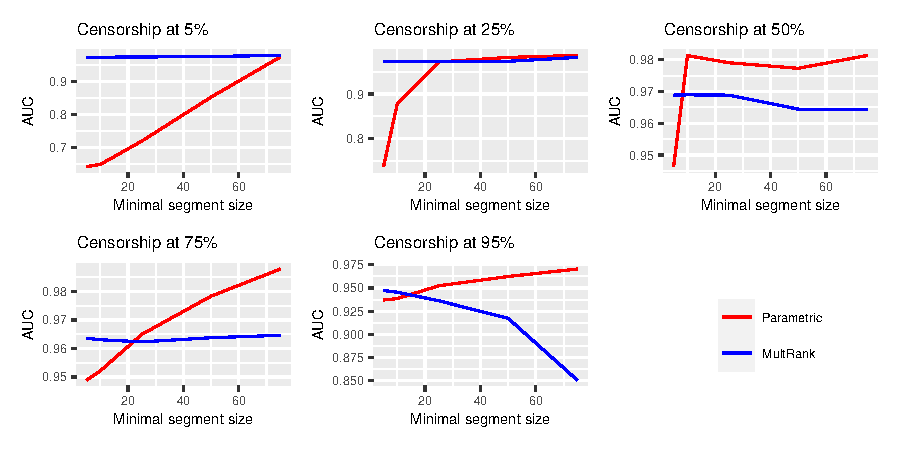
\includegraphics{figs/Chap4/sim_minseg.pdf}
    \caption{Choice of the minimal segment length: simulation results. Our method performance is Illustrated with the red line, the \textit{Multrank} method is drawn in blue. The results are illustrated for several censorship thresholds and the different minimal segment lengths used were $5,10,25,50$ and $75$ observations.}
    \label{fig:sim_minseg}
\end{figure}
    \item[$\blacksquare$] \textbf{The penalty calibration:} The last parameter to be set is the penalty $\beta$. While calibrating $\beta$, we want to compare the performance of the break detection with the Multrank method. The experimental framework is as follows: 
    \begin{enumerate}
        \item we simulate $N=100$ samples $(x_1,...,x_n)$ of size $n=400$  following a left-censored Weibull distribution with $\alpha\%$ of censored data. We made tests for the different censorship rates $\alpha = (25,50,75,95)$. The shape parameter of the Weibull distribution is assumed to be known and set to $\sigma=0.5$. The scaling parameters $\bm{\lambda^\star}$ have $K^\star=4$ breaks at positions $p^\star_1 = 80$, $p^\star_2 = 160$, $p^\star_3 = 240$ and $p^\star_4 = 320$ and take the values $\bm{\lambda^\star}=(\lambda^\star_1 = 1, \lambda^\star_2 = 4, \lambda^\star_3 = 0.5, \lambda^\star_4 = 5, \lambda^\star_5 = 1)$. An example of a sample simulated in this way is shown in Figure \ref{fig:ex_sim}.
        \item For each of the $N$ samples, we perform the parametric change-point detection and the Multrank methods. For each sample, we obtain the estimated number of breaks $\hat K_{param}$ and $\hat K_{multrank}$ and their position $(\hat{p}_{k,param})_{k = 1}^{\hat K_{param}}$ (respectively $(\hat{p}_{k,multrank})_{k = 1}^{\hat K_{multrank}}$).
        \item for both methods, we count the number of samples among the $N$ for which the correct number of breaks has been estimated (e.g. $\hat K_{param} = K^\star$). Also, for each of the samples for which the estimate of $K^\star$ is correct, we examine the distance between the estimated position of a change-point and its nearest true break $\min_{k,i \in [1:K^*]}(\hat{p}_{k} - p^\star_i)$. 
    \end{enumerate}
    In the case where $K$ is not known, we proceed as follows for each method to estimate it:
    \begin{itemize}
        \item For the parametric method: we use the algorithm CROPS, algorithm to scan a continuous range of penalty values $[\beta_{min},\beta_{max}]$. We obtain a set of $B$ values $(\hat \beta_1,...,\beta_B)$ and the optimal segmentations associated with these penalty values. We then plot the cost of the segmentations as a function of the number of breaks. We choose the optimal penalty using a elbow heuristic. This procedure is described in \cite{haynes2014}. The choice of $\beta_{min}$ and $\beta_{max}$ is inspired from linear penalties like the BIC criterion \cite{YAO1988181}. Note that when using the BIC penalty in change point detection, the penalty term written in section \ref{sub:pelt} becomes : $\beta_n = \frac{D}{2}\log(n) = \frac{1}{2}\log(n)$, where $D$ is the number of dimensions of the parameter. More precisely, we took a wide interval of penalty values defined by $\beta_{min} = \frac{\log(n)}{10}$ and $\beta_{max} = 5\log(n)$.
        \item For the non parametric \textit{Multrank} method, we compute the optimal segmentation for $k$ breaks, where $k$ ranges from $1$ to $K_{max}$. For each of these segmentations, we can compute the value of the statistic $I_k(n)$ statistic described in \cite{lung2015}. As in the parametric method, we represent the values of this statistic as a function of $k$, and we determine the number of estimated breaks by an elbow heuristic. Here, $K_{max}$ is fixed at $2*K^\star = 8$.
    \end{itemize}
The results of the simulations are shown in Table \ref{tab:simcomp} and in Figure \ref{fig:prec_sim}. It can be seen that in the ideal scenario, where the data are indeed distributed according to a left-censored Weibull distribution, the parametric method performs better both in detecting the correct number of breaks and in accurately estimating their position. However, this performance decreases as the censoring rate increases.

\begin{figure}[ht]
    \centering
    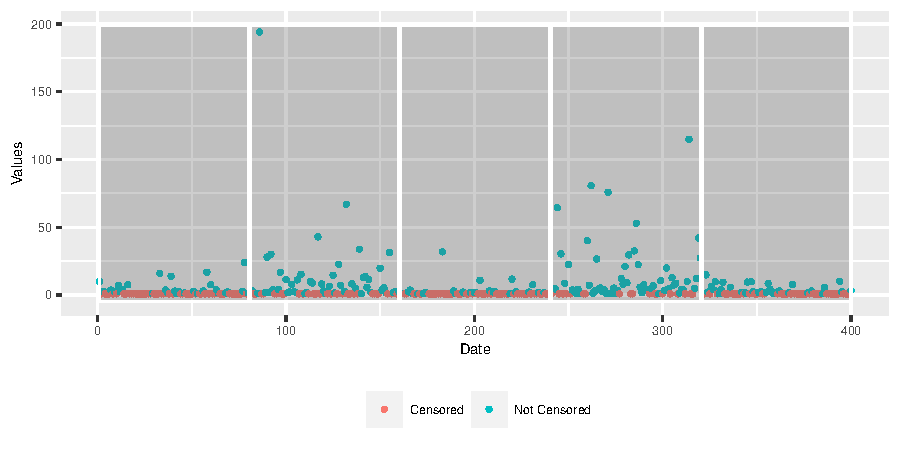
\includegraphics{figs/Chap4/Ex_sim.pdf}
    \caption{Example of simulated signal with $(\lambda_1 = 1, \lambda_2 = 4, \lambda_3 = 0.5, \lambda_4 = 5, \lambda_5 = 1)$, $\sigma = 0.5 $, $n = 400$, $K = 4$, $(p_1 = 80,p_2 = 160,p_3 = 240,p_4 = 320)$ and $\alpha = 50\%$.}
    \label{fig:ex_sim}
\end{figure}

\begin{table}[ht]
\centering
\begin{tabular}{|r|r|r|}
  \hline
   $\alpha(\%)$  & Parametric method & MultRank \\ 
  \hline
 25 &  84 &  58 \\ 
 50 &  80 &  63 \\ 
 75 &  87 &  68 \\ 
 95 &  65 &  10 \\ 
   \hline
\end{tabular}
\caption{Number of correct estimations of $K$ over $N=100$ samples for both methods for different $\alpha\%$ censorship rates.}
\label{tab:simcomp}
\end{table}

\begin{figure}[ht]
    \centering
    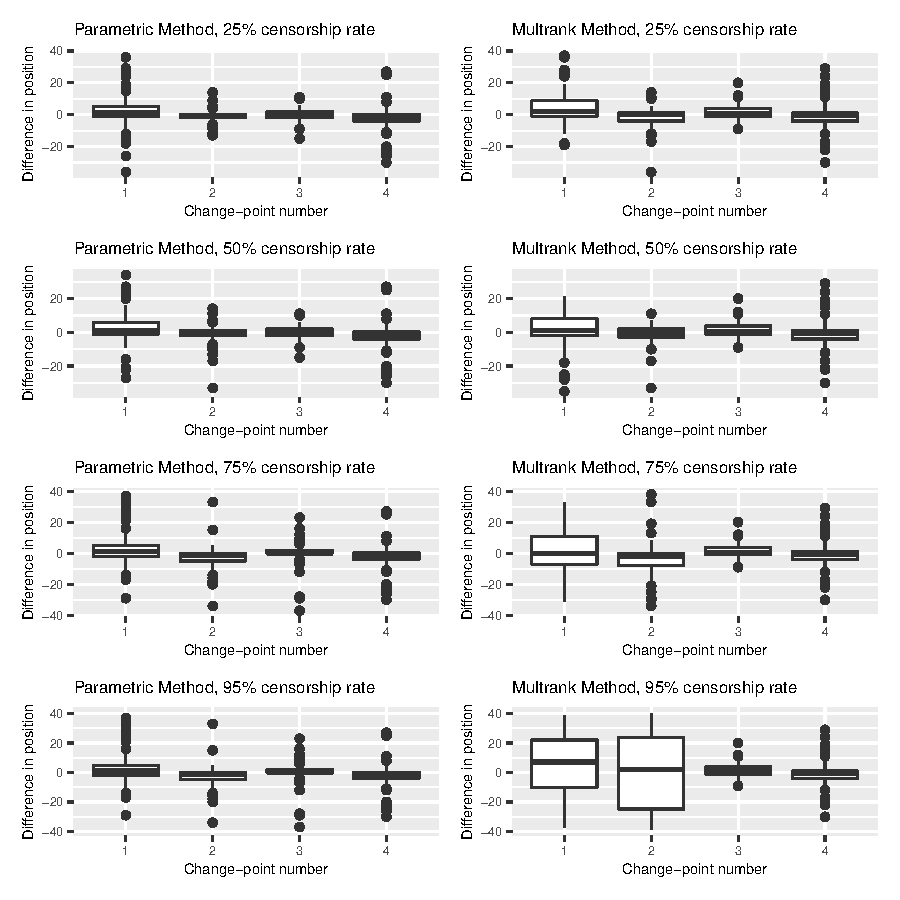
\includegraphics{figs/Chap4/P_RUPT.pdf}
    \caption{Precision of the estimated change-points for both methods.}
    \label{fig:prec_sim}
\end{figure}

\end{itemize}
